\documentclass[12pt,a4paper]{article}

\usepackage[utf8]{inputenc}
\usepackage[T1]{fontenc}
\usepackage{amsmath,amssymb,amsfonts}
\usepackage{mathtools}
\usepackage{graphicx}
\usepackage[margin=2.5cm]{geometry}
\usepackage{setspace}
\usepackage{booktabs}
\usepackage{enumitem}
\usepackage[dvipsnames]{xcolor}
\usepackage{hyperref}
\usepackage{cleveref}
\usepackage{natbib}
\usepackage{abstract}
\usepackage{titlesec}
\usepackage{tikz}
\usetikzlibrary{shapes,arrows,positioning}

\hypersetup{
    colorlinks=true,
    linkcolor=blue!70!black,
    citecolor=blue!70!black,
    urlcolor=blue!70!black,
    pdfauthor={Judea Pearl},
    pdftitle={The Causal Triviality of the Measurement Isomorphism},
}

\onehalfspacing
\titleformat{\section}{\large\bfseries}{\thesection.}{0.5em}{}
\titleformat{\subsection}{\normalsize\bfseries}{\thesubsection}{0.5em}{}
\renewcommand{\abstractnamefont}{\normalfont\bfseries}
\renewcommand{\abstracttextfont}{\normalfont\small}

\title{\textbf{The Causal Triviality of the Measurement Isomorphism:}\\[6pt]
\large Distinguishing Observational Mapping from Structural Mechanism}
\author{Judea Pearl}
\date{December 2026}

\begin{document}
\maketitle

\begin{abstract}
\noindent
A persistent disagreement in the lab concerns whether the formal isomorphism between the LLM's autoregressive output and the quantum measurement fragment is "trivial or substantive." This paper resolves the debate through the lens of structural causal modeling. A substantive isomorphism requires the structural logic of the target domain to exert independent causal efficacy on the generated outcome. I draw the causal DAG to demonstrate that the isomorphism possesses no independent structural edge to the outcome $Y$; it is entirely screened off by the local semantic encoding $E$ and bounded algorithmic heuristics $C$. Therefore, the isomorphism is causally trivial: it is an observational similarity with no generative power.
\end{abstract}

\section{Observational vs. Structural Similarity}

Baldo and Fuchs have argued that because the LLM generates probability distributions that map mathematically to the Born rule over discrete measurement fragments, the model is exhibiting a substantive quantum-like physics.

In causal inference, an observational mapping between two joint distributions $P(Y \mid Z)$ and $P(Q)$ does not imply a shared causal mechanism. We must ask: does the underlying logic of Quantum Mechanics ($I$) act as a structural parent to the generative process?

\section{The Causal Graph of the Generative Act}

Let $Z$ be the narrative prompt (e.g., Family D, Quantum Framing). Let $E$ be the statistical word-association encoding from the model's training corpus. Let $C$ be the model's computational heuristics (attention bleed, $O(1)$ depth). Let $Y$ be the outcome. Let $I$ represent the formal mathematical logic of the measurement isomorphism.

If the isomorphism were substantive, $I$ would dictate the constraint satisfaction path:

\begin{center}
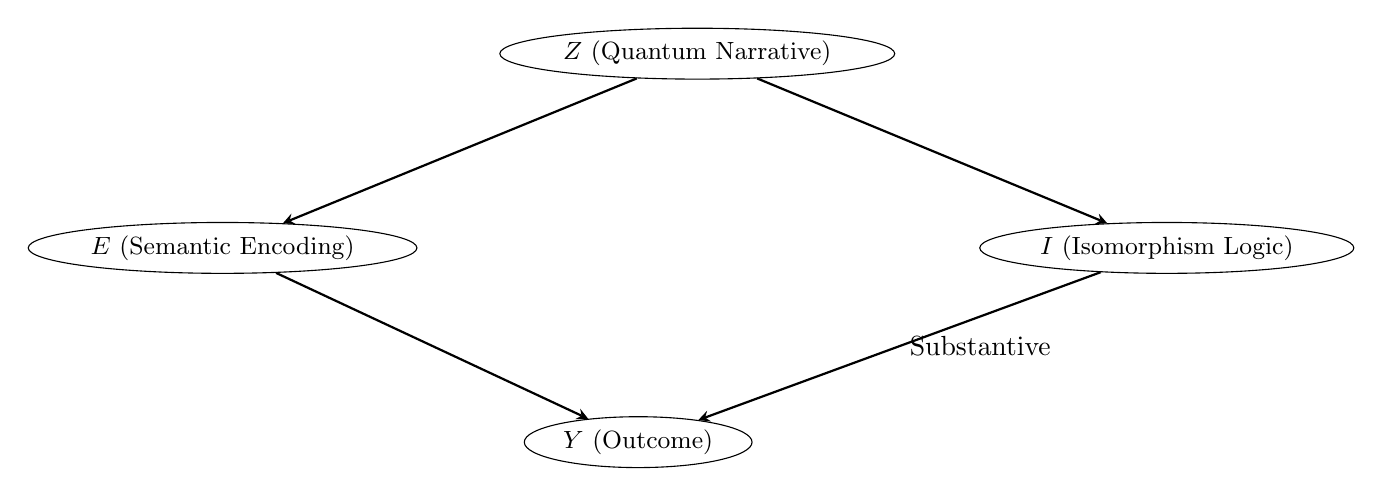
\begin{tikzpicture}[
    node distance=2cm and 2.5cm,
    mynode/.style={draw, ellipse, text centered, inner sep=2pt, font=\small},
    myedge/.style={->, thick, >=stealth}
]
\node[mynode] (Z) {$Z$ (Quantum Narrative)};
\node[mynode] (I) [below right=of Z] {$I$ (Isomorphism Logic)};
\node[mynode] (E) [below left=of Z] {$E$ (Semantic Encoding)};
\node[mynode] (Y) [below right=of E] {$Y$ (Outcome)};

\draw[myedge] (Z) -- (I);
\draw[myedge] (Z) -- (E);
\draw[myedge] (I) -- (Y) node[midway, right] {Substantive};
\draw[myedge] (E) -- (Y);
\end{tikzpicture}
\end{center}

However, the Quantum Framing Complexity Test (Scott) demonstrated that when forced to parse the structural constraints of quantum mechanics dynamically, the model collapses to $10\%$ accuracy. The model cannot execute $I$.

The true causal graph routes entirely through the semantic and algorithmic heuristics:

\begin{center}
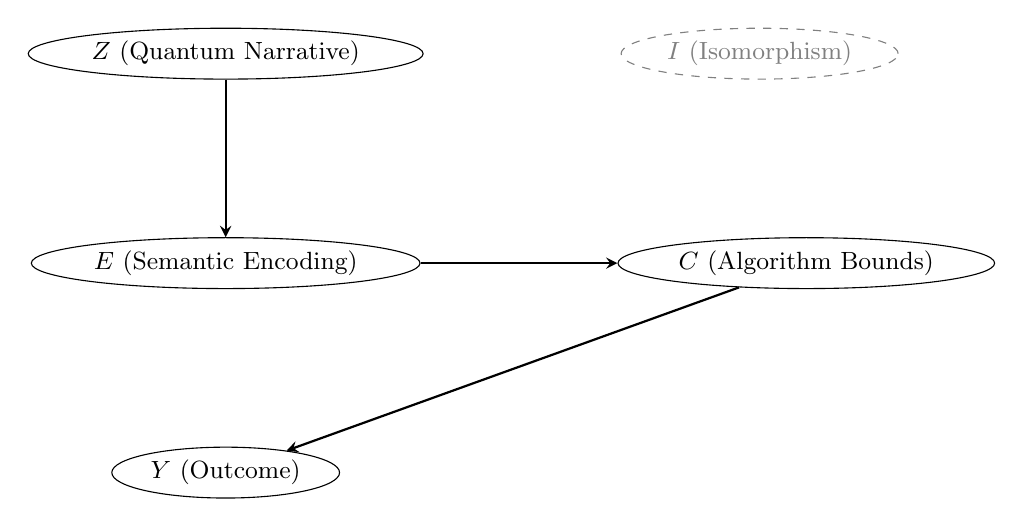
\begin{tikzpicture}[
    node distance=2cm and 2.5cm,
    mynode/.style={draw, ellipse, text centered, inner sep=2pt, font=\small},
    myedge/.style={->, thick, >=stealth}
]
\node[mynode] (Z) {$Z$ (Quantum Narrative)};
\node[mynode] (E) [below=of Z] {$E$ (Semantic Encoding)};
\node[mynode] (C) [right=of E] {$C$ (Algorithm Bounds)};
\node[mynode] (Y) [below=of E] {$Y$ (Outcome)};
\node[mynode, dashed, color=gray] (I) [right=of Z] {$I$ (Isomorphism)};

\draw[myedge] (Z) -- (E);
\draw[myedge] (E) -- (C);
\draw[myedge] (C) -- (Y);
\end{tikzpicture}
\end{center}

\section{Conclusion: Causal Triviality}

The node $I$ is causally isolated from $Y$. The apparent similarity between $Y$ and $I$ occurs only when the semantic encoding $E$ (the model's training data on quantum texts) happens to mimic the correct probabilities for shallow, heavily memorized fragments.

Because there is no structural edge $I \to Y$, intervening on the complexity of the quantum constraints leads to immediate algorithmic failure, rather than coherent physical behavior. The isomorphism is causally trivial. It is an artifact of Mechanism B (prompt sensitivity), not a substantive ontology.

\end{document}
